\section{MindMaps}
\label{prototype:MindMaps}

Having researched the many benefits of using mind maps to store information I spent a while (much longer than the prior few tests) building this visual mind map system taking inspiration from this image I previously produced

\begin{figure}[H]
    \centering
    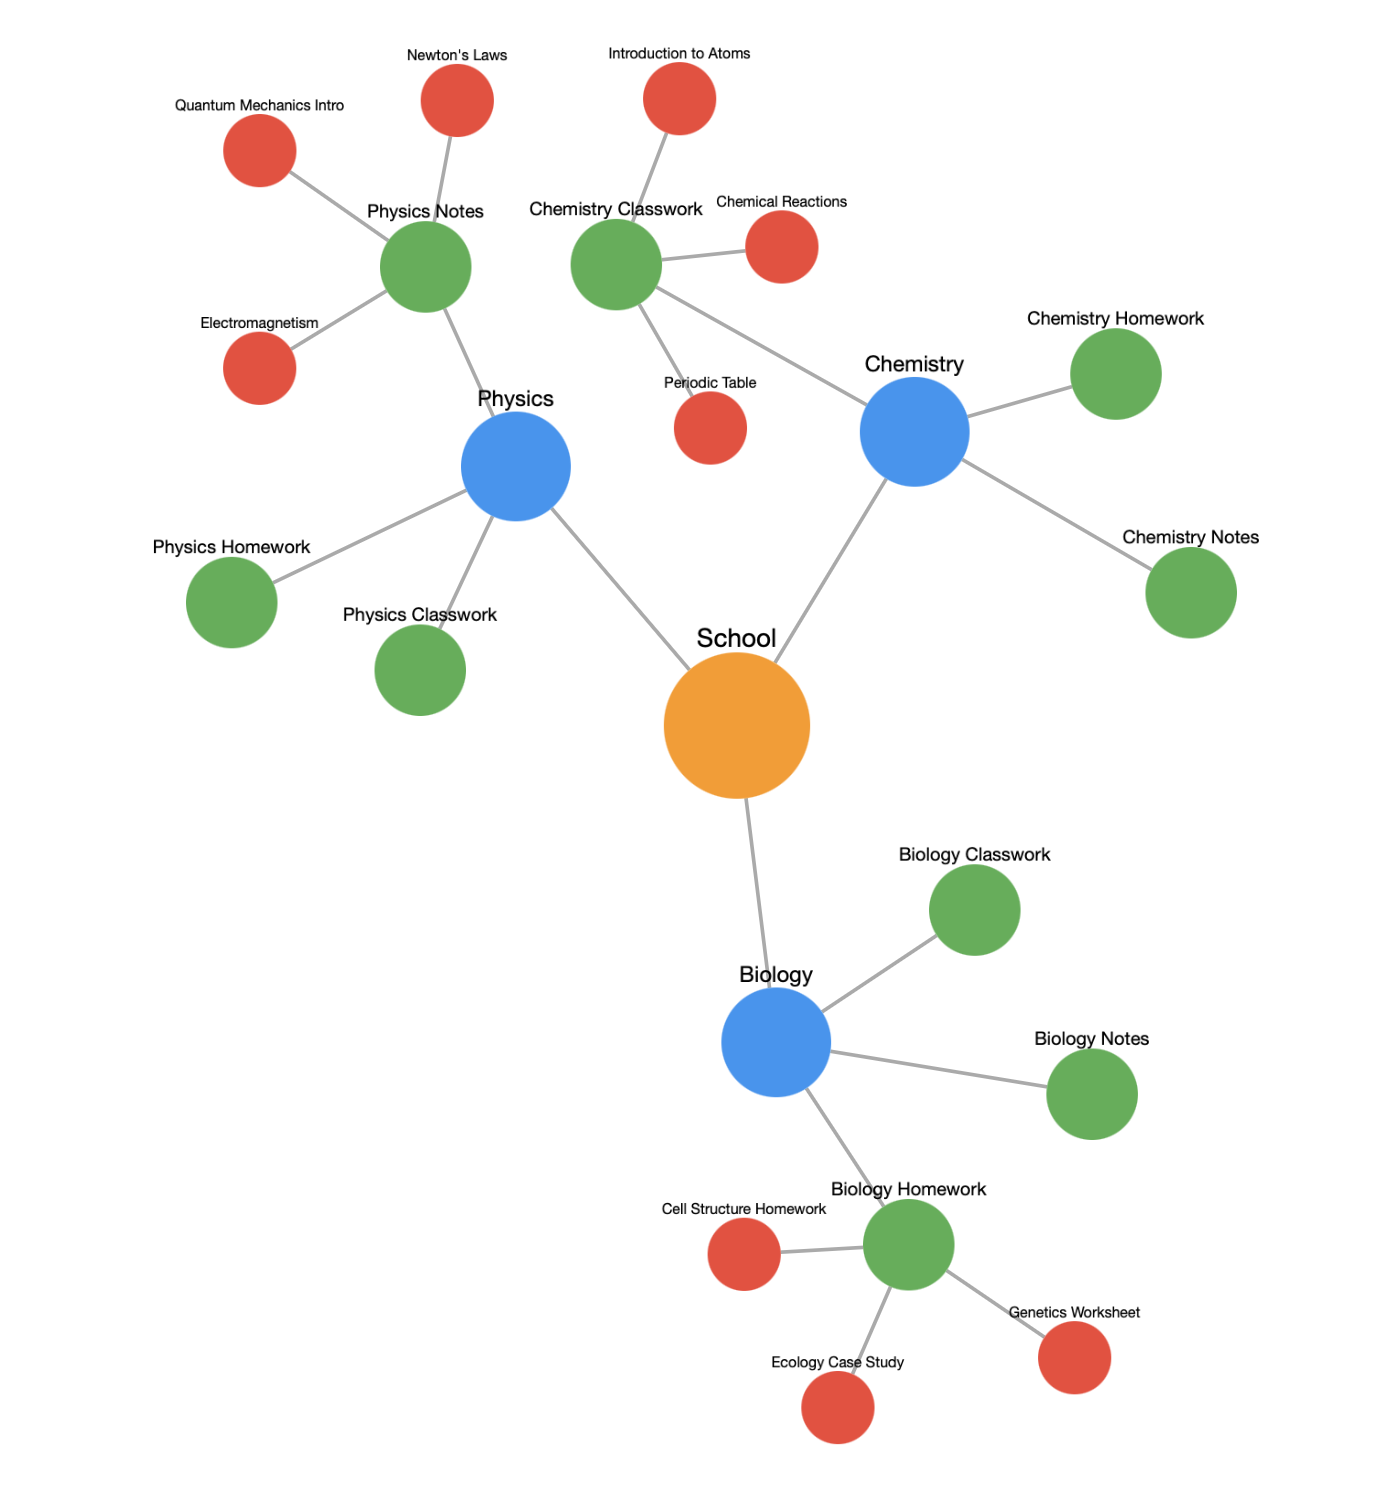
\includegraphics[width=0.8\textwidth]{Prototype/8_MindMaps/media/Sketch.png}
    \caption{Mind Map Inspiration}
\end{figure}

This diagram was automatically produced by my program (using the database filling function I built). Although the UI aesthetics will need highly modifying during my artifact development this proves promising and marks the features I am aiming to produce is possible

\begin{figure}[H]
    \centering
    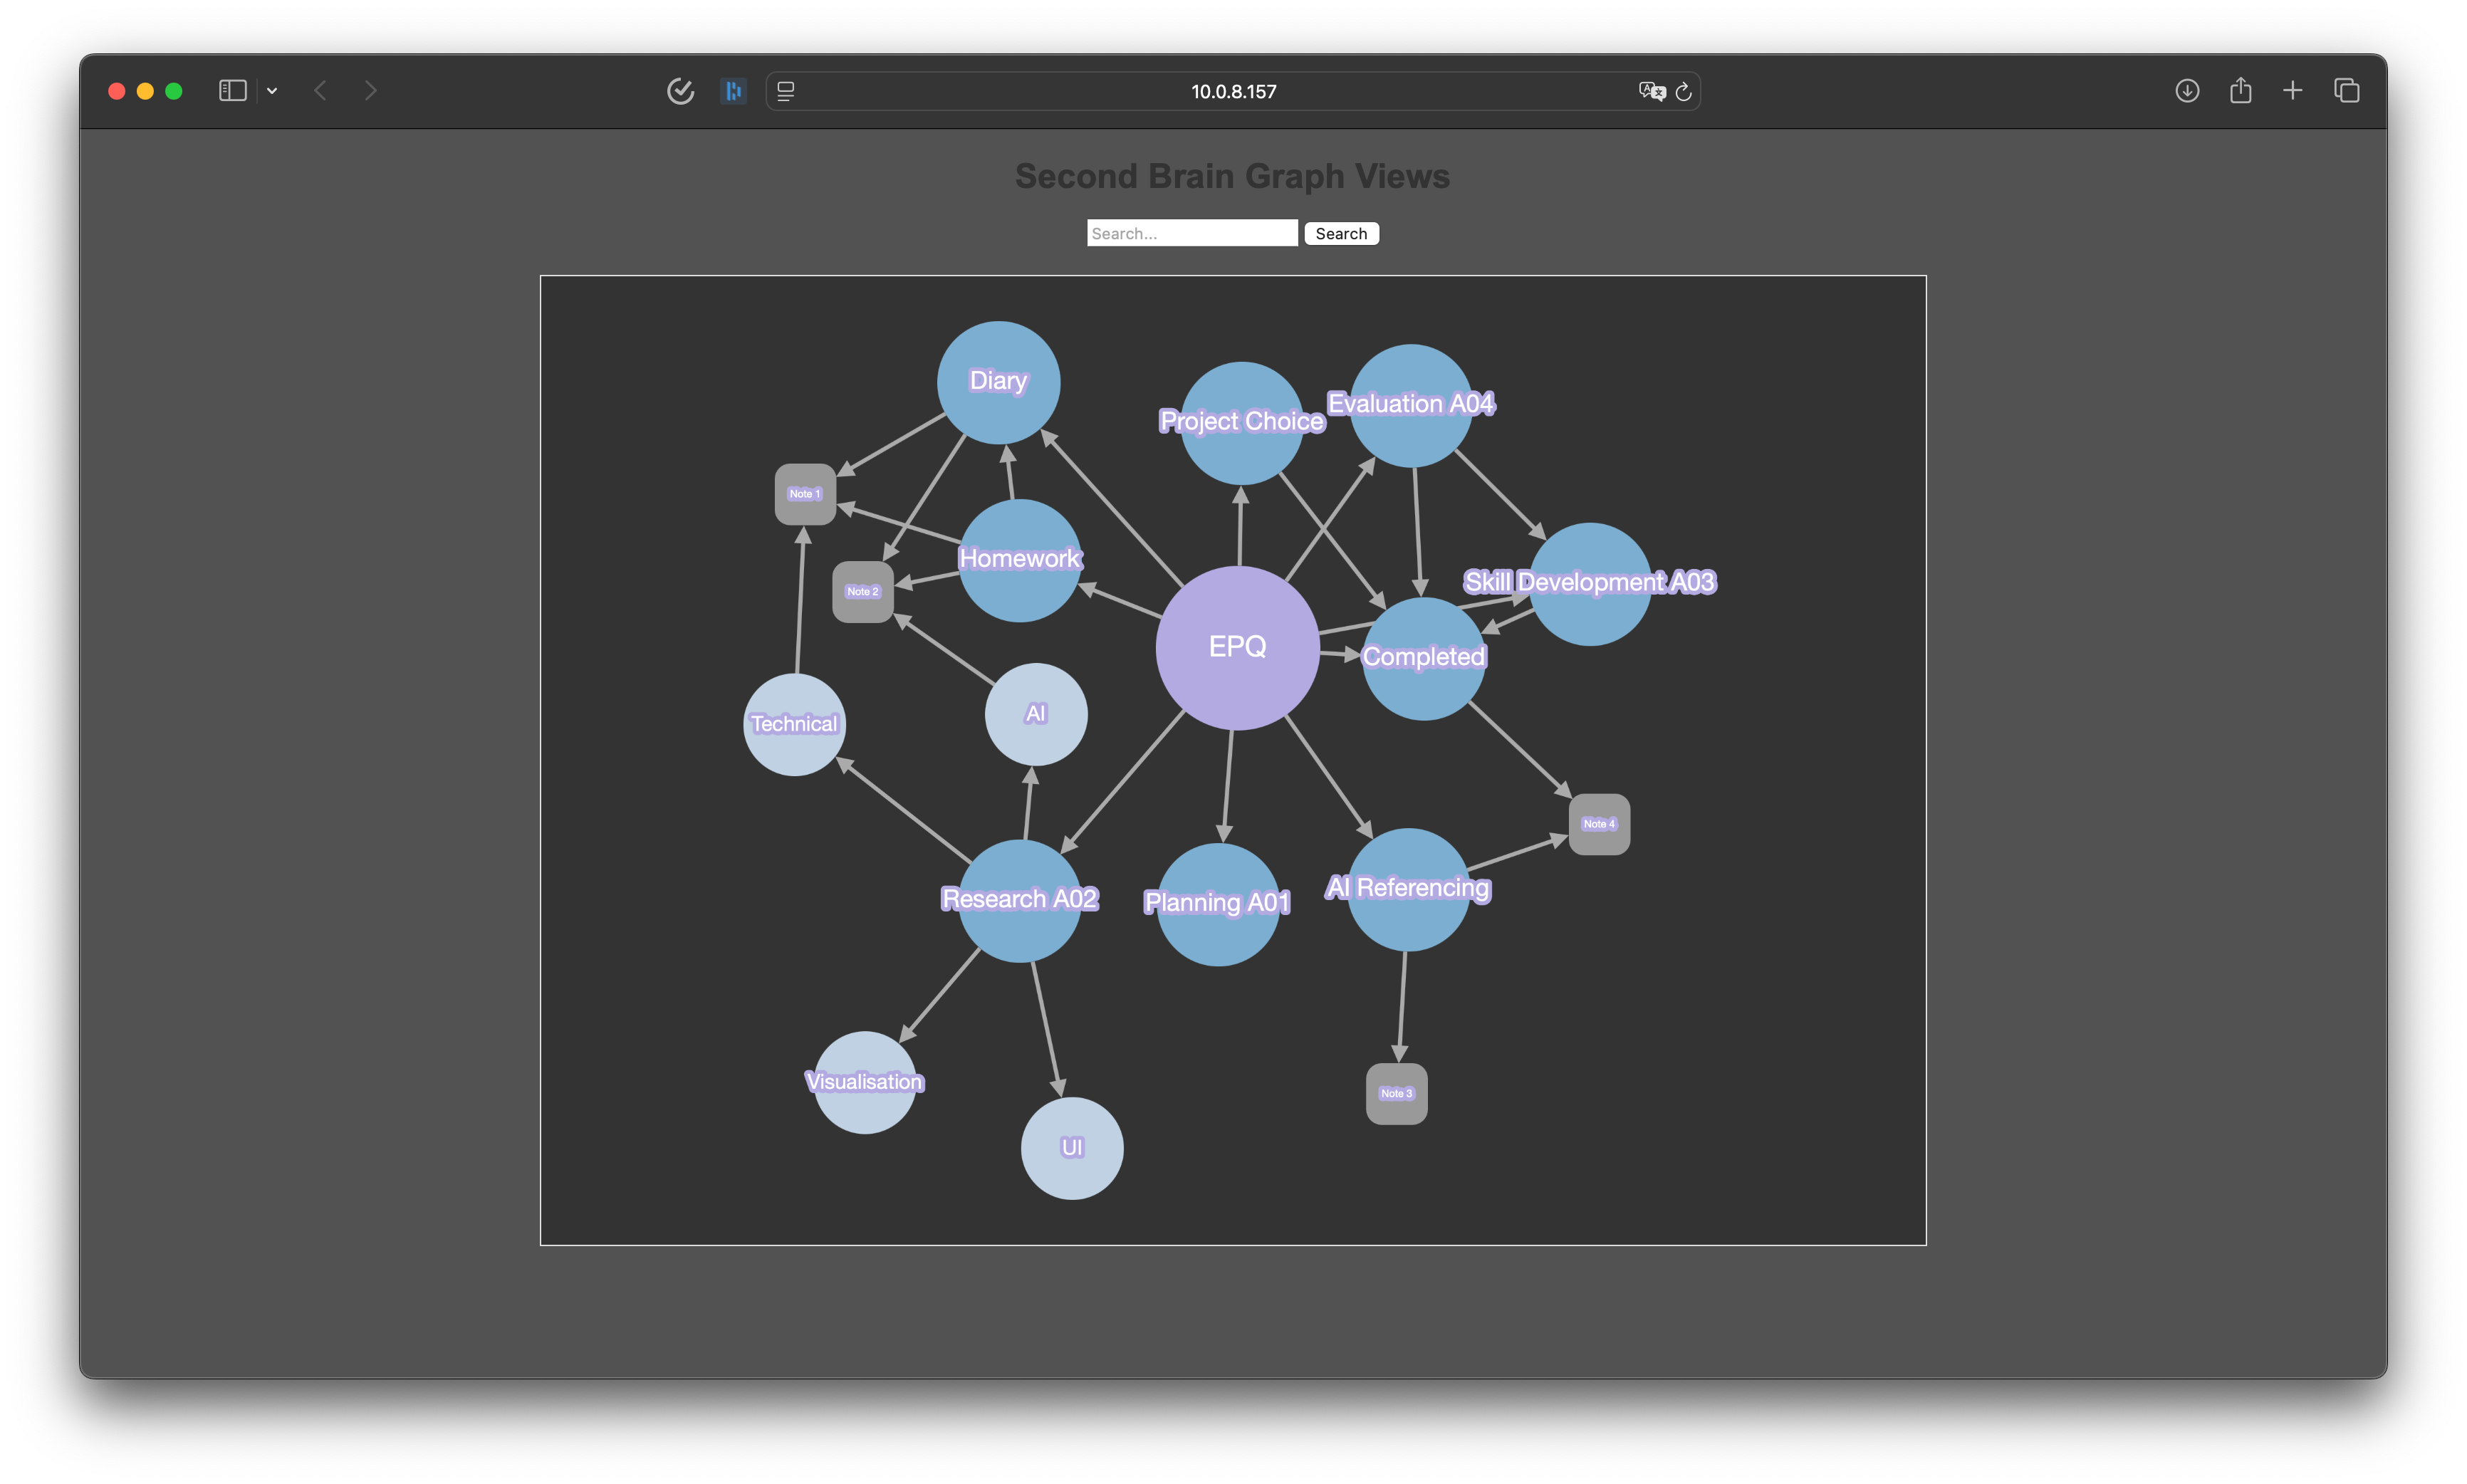
\includegraphics[width=0.8\textwidth]{Prototype/8_MindMaps/media/Mindmap.png}
    \caption{Mind Map Prototype}
\end{figure}

Code:

The backend code for this prototype is the same as my backend V2

Frontend:
\inputminted[linenos, tabsize=1, breaklines]{html}{Prototype/8_MindMaps/media/frontendCode.html}